%% Experimental report (King County) -- CSCE 3602 / DSCI 3415 Fundamentals of Machine Learning
%% AI was used to help write this report and its code; the authors reviewed and edited every part (Section 10).
%% Red [brackets] = a note for the authors, removed before submission.
\documentclass[sigconf,nonacm,10pt]{acmart}
\usepackage{tabularx}
\usepackage{booktabs}
\sloppy
\settopmatter{printacmref=false}
\setcopyright{none}
\renewcommand\footnotetextcopyrightpermission[1]{}
\pagestyle{plain}

\newcommand{\pending}[1]{\textcolor{red}{[#1]}}
\newcolumntype{Y}{>{\raggedright\arraybackslash}X}
\newcolumntype{L}[1]{>{\raggedright\arraybackslash}p{#1}}

\begin{document}

\title{Fair Price in a Moving Market: Predicting Residential Prices}
\subtitle{Experimental Report: Supervised Models on King County Home Sales}

\author{Zeyad Khaled}
\affiliation{%
  \institution{The American University in Cairo}
  \city{Cairo}
  \country{Egypt}}

\author{Mohamed Akram}
\affiliation{%
  \institution{The American University in Cairo}
  \city{Cairo}
  \country{Egypt}}

\begin{abstract}
We compare the supervised models covered in the course on 532,890 recorded home sales in King County, Washington, the county that contains Seattle, from 2000 onwards. The label is the natural log of the sale price. The dataset replaces the Zillow file of the first two phases, whose label was an assessed value rather than a price, and it was built to answer each comment on those phases (Section~\ref{sec:feedback}). Each sale is described by 55 features, which expand to 1,604 model columns. Every model followed one protocol: a five-fold search for its settings on 426,135 training sales, one final fit on all of them, and a single score on 106,755 test sales that played no part in any choice. On the test sales the neural network explained 94.7\% of the variation in log price and missed the typical home by 8.5\%. The random forest (91.2\%, 9.7\%) and bagging (91.0\%, 9.5\%) came next, ahead of linear regression (90.1\%, 12.9\%). We choose the neural network, and we report where it is unstable: its five validation folds vary six times more than the forest's.
\end{abstract}

\keywords{model comparison, cross-validation, regression, house prices, King County}

\maketitle

%% ---------------------------------------------------------------------------------------------------------------
\section{Response to the Phase 1 and Phase 2 Feedback}
\label{sec:feedback}

Both earlier phases lost marks. Studying the comments led us further than patching the Zillow pipeline: the Zillow label is the county's assessed value, which in California follows the price paid at the last sale rather than the home's market value \cite{prop13}, and the Zillow licence covers only a competition that closed in 2018 \cite{zillowprize2017}. The King County assessor publishes the recorded price of every sale, free to download \cite{kcassessor}. We moved to that data and rebuilt every step with the comments in mind. Table~\ref{tab:feedback} pairs each comment with what this study does about it.

\begin{table*}[t]
\caption{Each comment from the first two phases, what this study does about it, and the number that supports the decision. Association values are measured on training sales (Section~\ref{sec:checks}).}
\label{tab:feedback}
\small
\renewcommand{\arraystretch}{1.2}
\begin{tabularx}{\textwidth}{@{}L{3.6cm}YY@{}}
\toprule
Comment (phase) & What this study does & Evidence \\
\midrule
Dataset too small; limits of the data not discussed (Phase 1) & Public assessor records of every recorded sale since 2000, joined to the house, parcel and lookup files. Section~\ref{sec:limits} states the limits. & 532,890 sales of about 329,000 homes; 151 raw columns. \\
Label not a market price (found by us after Phase 2) & The label is now the recorded sale price, not an assessed value. & Zillow's label follows the last purchase price under Proposition 13; King County's is the price paid. \\
What is FIPS? Codes left unexplained (Phase 2) & Every numeric code is replaced by its name from the assessor's lookup file, and each of the 151 columns has a written meaning and decision. & 151 decisions, each with its measured reason. \\
Raw latitude and longitude used as inputs (Phase 2) & The survey grid became miles north and east. Both were dropped by the pair rule, and location enters through named areas, subdivisions and streets instead. & 0.998 and 0.996 with the appraisal area and sub-area. \\
City, county and region dropped (Phase 2) & Every location column was measured. Appraisal area + sub-area (299 codes) is kept; city and appraisal area lost to it under the pair rule; ZIP code was removed with a measured reason. The whole dataset is one county. & Area + sub-area 0.594 with the label; city 0.868 with it; ZIP code adds 4.0 points of explained price on top of the appraisal area, against 5.7 for the sub-area. \\
No distribution analysis; log taken with no analysis (Phase 2) & Figure~\ref{fig:distributions} shows the price and the living area before and after the log, with the skew of each, and the log is justified by the share of error the most expensive sales carry. & Price skew 6.15 falls to 0.47; the top 1\% of sales carry 44.9\% of squared dollar error and 9.9\% after the log. \\
A decision with no number, for every feature (Phase 2) & Each column was measured on the training sales: a table of its values, the share of price differences it explains, and its correlation with the label. & 55 features kept, five dropped by the pair rule (Appendix~\ref{app:features}). \\
Text features (professor's rule on text) & Subdivision names, street names and street types are one-hot encoded. Zoning was removed with a measurement, because the same code means different rules in different cities. & 800, 404 and 15 model columns. Zoning: 399 codes, median 30 sales per code. \\
AI use not declared (Phases 1 and 2) & Section~\ref{sec:ai} states how AI was used, and every code file opens with the same statement. & Every script carries the statement. \\
References not cited (Phases 1 and 2) & Every method, library and data source is cited where it is used. & 19 references. \\
\bottomrule
\end{tabularx}
\end{table*}

%% ---------------------------------------------------------------------------------------------------------------
\section{Data}
\label{sec:data}

\subsection{The files and the label}
The King County Department of Assessments publishes four extracts \cite{kcassessor}: one row per recorded sale, one per residential building, one per parcel of land, and a lookup file with the names behind the numeric codes. They join on the parcel number and together hold 151 columns. We treat a home's price as the sum of what its characteristics are worth, the hedonic view of housing \cite{rosen1974hedonic}.

The label is the natural log of the sale price. The median training sale is \$505,000 and the largest \$32 million, so the raw price has a skew of 6.15 (Figure~\ref{fig:distributions}). In dollars, the most expensive 1\% of training sales carry 44.9\% of the squared error of a model, which would spend its effort on mansions. After the log they carry 9.9\% and the skew falls to 0.47. A miss on the log scale behaves like a percentage miss, so being 10\% off counts the same on a \$300,000 house and on a \$3 million one. Every dollar figure in this report converts the log prediction back with the exponential.

\begin{figure*}[t]
\centering
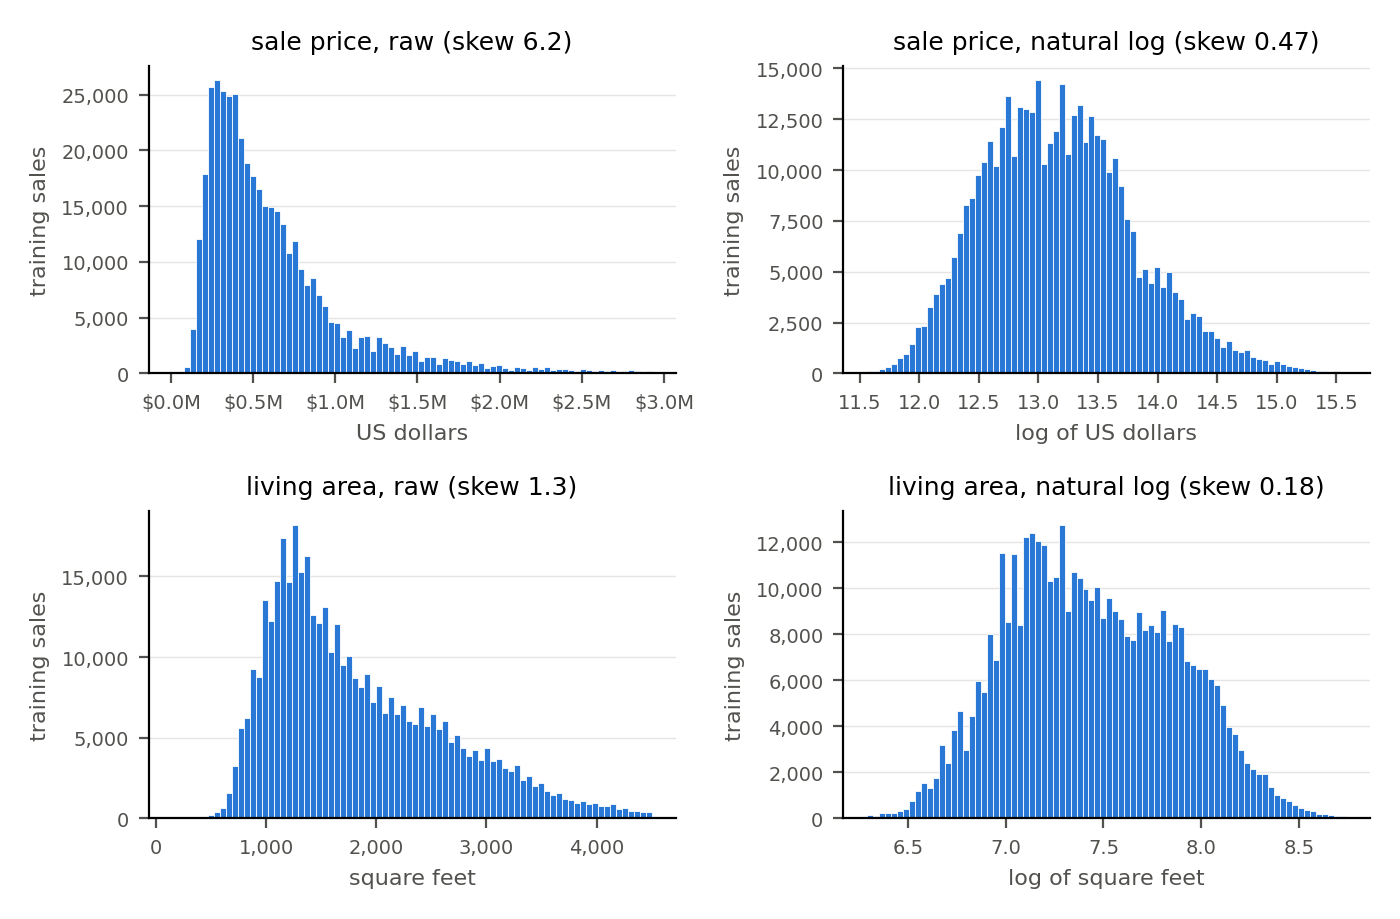
\includegraphics[width=0.82\textwidth]{figures/distributions.png}
\caption{The sale price (top) and the above-ground living area (bottom) of the 426,135 training sales, raw and after the natural log. Raw panels stop at the 99th percentile (\$2.93 million and 4,500 square feet) so the bars stay visible; log panels drop the outer 0.1\% on each side. Each skew is computed on every training sale.}
\label{fig:distributions}
\end{figure*}

\subsection{Which sales are kept}
A sale counts only if it is an ordinary market sale of one house. The rules are:
\begin{itemize}
\item no special circumstance recorded, and a warranty or statutory warranty deed;
\item no sale warning, and only one parcel in the sale;
\item residential use, on residential land with a building;
\item a price of at least \$10,000, sold in 2000 or later;
\item exactly one house on the parcel, not built or renovated after the sale;
\item at least one bedroom and one bathroom.
\end{itemize}
The first five rules leave 533,055 sales of 328,776 homes. The last removes 165 more, leaving 532,890. Buyer and seller names were removed at the start: they are personal data, the county's terms restrict the use of lists of individuals, and a name says nothing about the house.

\subsection{Training sales, test sales and folds}
Many houses sold more than once. If one sale of a house sat in training and a later sale of the same house in the test set, a model could recognise the house instead of pricing it. The split is therefore by home, with seed 42: 426,135 training sales and 106,755 test sales, with every sale of one house on the same side. The test sales were sealed, and each final model was scored on them once.

The training sales were divided by home into five folds of 85,226, 85,272, 85,615, 84,937 and 85,085 sales. Every model used the same five folds, so all models are compared on the same homes.

\subsection{Features}
The 55 features expand to 1,604 model columns: 17 standardized numbers (minus the training average, divided by the training spread), 23 yes/no columns, and 1,564 one-hot columns. Appendix~\ref{app:features} lists them by group. The main ones are the above-ground living area (log), the building grade, the bathrooms and bedrooms, the year built, ten view columns, the waterfront, and the sale date as years since 1 January 2000 with decimals, which lets the models learn how the market moved.

Location enters as names. The appraisal area joined with its sub-area gives 299 codes. Subdivision names with at least 100 training sales get their own column (800 columns), as do street names with at least 200 sales (404 columns); every rarer name shares one ``other'' column, because a name seen a dozen times cannot teach a reliable price. In every category, values under 0.1\% of training sales are grouped, and the most common value is dropped as the baseline. All of these lists and thresholds were learned from the training sales only.

\subsection{Correlation checks}
\label{sec:checks}
Association was measured by the Pearson correlation for two numbers, by the correlation ratio for a category and a number, and by the bias-corrected Cram\'er's V for two categories \cite{cramer1946,bergsma2013}. Columns with many names were measured on held-out homes: fitted on four of every five homes and scored on the fifth, so that a column with thousands of names could not score itself on its own homes. Figure~\ref{fig:heatmap} in the appendix shows the 60 candidate features.

The rules ran in this order.
\begin{enumerate}
\item When two features reach 0.85 with each other, the one weaker with the label is dropped, strongest pair first. Five went: appraisal area (1.000 with area + sub-area), miles north (0.998), miles east (0.996), tidelands or shorelands (0.986 with which water the house is on) and city (0.868 with area + sub-area).
\item No feature may reach 0.85 with the label (the professor's rule). None did; the strongest is the sale date at 0.641.
\item A dropped column comes back if it lies between 0.60 and 0.80 with the label and stays under 0.85 with every kept feature. Only the parcel number (0.662) fell in that window, and it is 0.998 with miles north, so nothing came back.
\item One baseline column was dropped per category group, 15 in all.
\item Among the model columns, two subdivision columns that copied a sub-area column were dropped. The smallest eigenvalue of the column correlation matrix is 0.0067, so no column is an exact combination of the others.
\end{enumerate}

%% ---------------------------------------------------------------------------------------------------------------
\section{Experimental Setup}
\label{sec:setup}

\subsection{One protocol for every model}
Every model went through the same four steps.
\begin{enumerate}
\item \textbf{Search.} Each setting trains on four folds (about 341,000 sales) and is scored on the fifth, five times, so every training home is checked once by a model that never saw it \cite{kohavi1995}.
\item \textbf{Winner.} The setting with the lowest average validation mean squared error (MSE) of the log price wins. A setting counts only if all five of its runs trained.
\item \textbf{Final fit.} The winner is trained once, from scratch, on all 426,135 training sales, 25\% more than any search run saw.
\item \textbf{Test.} The final model is scored once on the 106,755 test sales. The code refuses to score a model on them a second time.
\end{enumerate}
The selection works on MSE of the log price because most models minimise squared error, and on the log scale it measures relative misses. Linear regression has no setting to search but still ran on the five folds; the baselines were validated on fold 0.

\subsection{Scores}
For each model we report the MSE and the coefficient of determination ($R^2$) on the log price, $R^2$ and the root mean squared error (RMSE) in dollars, the median miss in dollars and as a percentage of the price, and the shares of homes predicted within 10\% and 20\% of their price. Dollar scores are dominated by the most expensive homes, which Section~\ref{sec:top} examines separately.

\subsection{Hardware and software}
Everything ran on an Apple M1 Pro laptop with 16 GB of memory, in Python 3.12 with scikit-learn 1.8 \cite{pedregosa2011} and PyTorch 2.11 \cite{paszke2019}. The neural network and the nearest-neighbour search ran on the laptop's graphics processor. Every random step uses seed 42 (or 42 plus the fold number).

\begin{table*}[t]
\caption{Every model, the lecture it comes from, the settings searched, what was held fixed, and the setting that won on validation.}
\label{tab:grids}
\small
\renewcommand{\arraystretch}{1.15}
\begin{tabularx}{\textwidth}{@{}L{2.6cm}L{0.9cm}YYL{3.1cm}@{}}
\toprule
Model & Lecture & Settings searched & Held fixed & Winner \\
\midrule
Average and median baselines & -- & none & one price for every home (\$663,874 or \$505,000) & -- \\
Linear regression & 4 & none & ordinary least squares, all 1,604 columns & -- \\
Neural network & 7 & hidden layers 128--64, 256--128, 512--256; dropout 0 or 0.2; SGD at learning rate 0.1 or Adam at 0.001 (12 settings) & ReLU; batch 1,024; MSE loss; at most 100 passes; stop after 5 passes without improvement & 256--128, SGD 0.1, dropout 0.2; 56 passes \\
K-nearest neighbours & 3 & $k$ = 1, 3, 5, 10, 15, 20, 30, 50; Euclidean or cosine distance (16 settings) & exact search; prediction = mean log price of the $k$ neighbours & cosine, $k$ = 15 \\
Decision tree & 10 & pruning strength 0, $10^{-7}$, $10^{-6}$, $3\times10^{-6}$, $10^{-5}$, $3\times10^{-5}$, $10^{-4}$ & squared-error splits; tree grown in full, then pruned by cost complexity & $3\times10^{-6}$ \\
Random forest & 10 & columns per split: square root (40), 10\% (160), 33\% (529) & 50 unpruned trees on bootstrap samples & 33\% of the columns \\
Bagging & 10 & none & 50 unpruned trees, every column at every split & -- \\
Support vector machine & 12 & penalty $C$ = 0.01 or 1; margin width $\epsilon$ = 0 or 0.05 (4 settings) & linear kernel; $\epsilon$-insensitive loss; at most 2,000 passes & $C$ = 1, $\epsilon$ = 0.05 \\
\bottomrule
\end{tabularx}
\end{table*}

\pending{Not run on this dataset, at your decision: AdaBoost, K-means and hierarchical clustering, voting, and the price-band classifiers (logistic regression, perceptron, naive Bayes). The Phase III brief asks regression projects to try classifiers on a binned label.}

%% ---------------------------------------------------------------------------------------------------------------
\section{The Models One by One}
\label{sec:models}

Each subsection gives the model's setup and why its settings were chosen, its validation and test results, and how well it fits the problem. Table~\ref{tab:test} collects the test scores.

\subsection{Baselines}
The average baseline predicts the average training price, \$663,874, for every home; the median baseline predicts \$505,000. On the test sales they miss the typical home by 51.0\% and 41.9\% (MSE of the log 0.466 and 0.417). The average baseline's $R^2$ on the log is negative ($-0.124$) because a few very expensive homes pull the average above what a typical home sells for. Any model worth keeping has to beat these numbers by a wide margin.

\subsection{Linear regression}
Ordinary least squares fits one weight per column \cite{hastie2009}, and each weight reads as ``this column adds a fixed percentage to the price''. The five fold scores lie between 0.0411 and 0.0415 (average 0.0412, spread 0.0002), the steadiest of any model. The fit on the homes it learned from ($R^2 = 0.902$) barely differs from the fit on held-out homes (0.900), so the model is not memorising. On the test sales it scored 0.0411 ($R^2 = 0.901$), a median miss of 12.9\% (\$65,423), with 40.0\% of homes within 10\% and 70.0\% within 20\%.

A straight line already explains nine tenths of the variation in log price, which says the features carry most of what sets a price. Its limit is that each column has one effect everywhere: a view of Lake Washington adds the same percentage in every area of the county. It fits in about five seconds, and every weight can be read and checked.

\subsection{Neural network}
The network is a fully connected feed-forward network trained by backpropagation \cite{rumelhart1986}: 1,604 inputs, two hidden layers with the ReLU activation, dropout after each hidden layer \cite{srivastava2014}, and one output for the log price. Training minimises the squared error in batches of 1,024 sales, reshuffled every pass, about 333 weight updates per pass. A run stops when the validation error has not improved for five passes, at most 100, and keeps the weights from its best pass.

We first tried Adam \cite{kingma2015} at a learning rate of 0.1 in a short trial, and its error rose after the first pass. The main search therefore ran plain stochastic gradient descent (SGD) at 0.1 on three sizes with and without dropout, and a second search ran Adam at its standard rate of 0.001 on the same six networks. Table~\ref{tab:nn} shows all twelve settings; the 60 runs took 81 minutes.

\begin{table}[t]
\caption{Neural network search: average over the five validation folds, best first. Spread is the standard deviation of the fold scores. The first two rows lost a fold and do not count.}
\label{tab:nn}
\small
\setlength{\tabcolsep}{3pt}
\begin{tabular}{@{}lrrrrr@{}}
\toprule
Setting & Folds & MSE & Spread & Median & Best \\
 & trained & (log) & & miss \% & pass \\
\midrule
512--256 SGD, drop 0 & 4 of 5 & 0.0192 & 0.0018 & 7.9 & 28 \\
512--256 SGD, drop 0.2 & 4 of 5 & 0.0203 & 0.0046 & 8.0 & 49 \\
\textbf{256--128 SGD, drop 0.2} & 5 of 5 & \textbf{0.0204} & 0.0031 & 8.1 & 56 \\
128--64 SGD, drop 0 & 5 of 5 & 0.0205 & 0.0014 & 8.2 & 18 \\
128--64 Adam, drop 0 & 5 of 5 & 0.0211 & 0.0012 & 8.2 & 29 \\
256--128 SGD, drop 0 & 5 of 5 & 0.0218 & 0.0064 & 8.4 & 27 \\
128--64 SGD, drop 0.2 & 5 of 5 & 0.0231 & 0.0043 & 8.7 & 49 \\
256--128 Adam, drop 0 & 5 of 5 & 0.0265 & 0.0062 & 9.4 & 29 \\
256--128 Adam, drop 0.2 & 5 of 5 & 0.0297 & 0.0105 & 10.3 & 38 \\
512--256 Adam, drop 0 & 5 of 5 & 0.0322 & 0.0069 & 10.6 & 37 \\
128--64 Adam, drop 0.2 & 5 of 5 & 0.0357 & 0.0106 & 11.6 & 28 \\
512--256 Adam, drop 0.2 & 5 of 5 & 0.0390 & 0.0231 & 11.5 & 39 \\
\midrule
\emph{Linear regression} & 5 of 5 & 0.0412 & 0.0002 & 12.9 & -- \\
\bottomrule
\end{tabular}
\end{table}

Both 512--256 SGD settings blew up on fold 1, where the error became infinite on the first pass. Their averages over the four surviving folds look better than the winner's, but an average that skips the failed run hides the failure, so by the protocol they do not count. The winner is 256--128 with dropout 0.2, trained by SGD. Adam at 0.001 did not beat SGD. Its best setting (128--64 without dropout, 0.0211) is the steadiest network, with a spread of 0.0012, while Adam's other settings were worse and uneven.

The final network trained from fresh weights on all training sales for 56 passes, the median best pass of its five runs, in 166 seconds. On the test sales it scored 0.0221 ($R^2 = 0.947$ on the log, 0.924 in dollars), missed the typical home by 8.5\% (\$40,511), and placed 57.2\% of homes within 10\% and 85.3\% within 20\%. That is 46\% less squared error than linear regression. The network can learn that the same feature is worth different amounts in different places, which no straight-line model can. Its costs are tuning, instability (Section~\ref{sec:top}) and a lack of explanation: it gives no weight a valuer can read.

\subsection{K-nearest neighbours}
A home is priced at the mean log price of the $k$ training sales closest to it in the 1,604-column space \cite{cover1967}. Each fold compares 85,000 checking sales with 341,000 training sales, about 29 billion distances, computed exactly on the graphics processor. Cosine distance compares the pattern of two rows and ignores their length; Euclidean distance is the straight-line distance.

One neighbour was the worst setting (0.139 Euclidean, 0.145 cosine), because a single sale's price is noisy. The error fell to its lowest at $k$ = 15 with cosine distance (0.0820, spread 0.0008) and rose again beyond it (0.0857 at $k$ = 50) as more distant homes were averaged in. Cosine beat Euclidean from $k$ = 5 up. On the test sales the final model scored 0.0798 ($R^2 = 0.808$) with a median miss of 16.8\%, the weakest of the trained models. Every column counts equally in the distance, so matching on an unimportant yes/no column counts as much as matching on living area. The search took 2.3 hours, and the process running it grew to 13 GB on the 16 GB laptop.

\subsection{Decision tree}
A regression tree (CART) splits the sales in two again and again to cut the squared error, and predicts the average log price in each leaf \cite{breiman1984}. We grew each tree in full and pruned it by cost complexity: a branch stays only if it lowers the squared error by at least the pruning strength for every leaf it adds. The full tree scored 0.0736. Light pruning helped, reaching 0.0598 at $10^{-6}$ and 0.0595 at $3\times10^{-6}$, the winner. Heavier pruning hurt: 0.0672 at $10^{-5}$ and 0.0883 at $10^{-4}$. Too little pruning learns the noise of a few sales per leaf; too much leaves too few leaves to tell neighbourhoods apart.

The final tree scored 0.0582 on the test sales ($R^2 = 0.860$), with a median miss of 13.9\%. A single tree reads like a set of rules and needs no scaling, but it is worse than a straight line here because its prediction jumps between leaf averages. Pruning was also slow: each pruned tree took about seven minutes against 39 seconds for the full tree.

\subsection{Random forest}
A random forest averages 50 trees, each grown on a bootstrap sample and allowed to split only on a random share of the columns at each split \cite{breiman2001}. A third of the columns (529) won with 0.0381 (spread 0.0005), ahead of 10\% (0.0401) and the square root, 40 columns (0.0529). Most of the 1,604 columns are location columns that are zero for almost every sale, so a random draw of 40 columns often contains nothing worth splitting on.

On the test sales the forest scored 0.0363 ($R^2 = 0.912$), with a median miss of 9.7\% and 51.2\% of homes within 10\%. It has a single setting worth tuning, and its folds agree closely. Against it: 50 full trees are large in memory, and the forest cannot predict above the most expensive sale in a leaf, which costs it at the top of the market (Section~\ref{sec:top}).

\subsection{Bagging}
Bagging is the same forest with every column available at every split \cite{breiman1996}, so its trees differ only through their bootstrap samples. It scored 0.0397 on validation (spread 0.0005) and 0.0374 on the test sales ($R^2 = 0.910$, median miss 9.5\%). The random choice of columns in the forest helps, but only slightly: the forest's trees are less alike, and their average gains a little more.

\subsection{Support vector machine}
A linear support vector machine for regression ignores misses smaller than a margin $\epsilon$ and penalises larger ones in proportion to their size, weighted by $C$ \cite{cortes1995}; we used the solver built for large linear problems \cite{ho2012}. A kernel version would need all 181 billion pairs of training sales, far beyond 16 GB. The four settings landed between 0.0416 and 0.0419, next to linear regression, since both are straight lines over the same columns. The winner ($C$ = 1, $\epsilon$ = 0.05) scored 0.0414 on the test sales ($R^2 = 0.900$, median miss 12.7\%). Fits at $C$ = 1 took about 150 seconds against 12 at $C$ = 0.01, and 11 of them did not fully converge in 2,000 passes; they still scored within 0.0003 of the rest. The absolute-error loss makes the line less sensitive to a few wild sales, which shows in a slightly lower median miss than linear regression.

%% ---------------------------------------------------------------------------------------------------------------
\section{All Models Side by Side}
\label{sec:all}

\begin{table*}[t]
\caption{Every model on the 106,755 test sales, ranked by average validation MSE of the log (the baselines on fold 0 only). Each model was scored on the test sales once.}
\label{tab:test}
\small
\begin{tabular}{@{}lrrrrrrrr@{}}
\toprule
Model & Validation & Test MSE & Test $R^2$ & Test $R^2$ & RMSE & Median & Within & Within \\
 & MSE (log) & (log) & (log) & (\$) & (\$) & miss (\%) & 10\% (\%) & 20\% (\%) \\
\midrule
Neural network & 0.0204 & 0.0221 & 0.947 & 0.924 & 161,546 & 8.5 & 57.2 & 85.3 \\
Random forest & 0.0381 & 0.0363 & 0.912 & 0.870 & 211,017 & 9.7 & 51.2 & 77.6 \\
Bagging & 0.0397 & 0.0374 & 0.910 & 0.872 & 209,399 & 9.5 & 51.7 & 77.4 \\
Linear regression & 0.0412 & 0.0411 & 0.901 & 0.885 & 197,716 & 12.9 & 40.0 & 70.0 \\
Support vector machine & 0.0416 & 0.0414 & 0.900 & 0.883 & 200,266 & 12.7 & 40.8 & 70.2 \\
Decision tree & 0.0595 & 0.0582 & 0.860 & 0.795 & 264,791 & 13.9 & 37.2 & 65.9 \\
K-nearest neighbours & 0.0820 & 0.0798 & 0.808 & 0.715 & 311,896 & 16.8 & 31.4 & 57.6 \\
Median baseline & 0.4174 & 0.4171 & $-0.006$ & $-0.077$ & 606,267 & 41.9 & 11.5 & 23.2 \\
Average baseline & 0.4663 & 0.4661 & $-0.124$ & 0.000 & 584,290 & 51.0 & 11.2 & 22.2 \\
\bottomrule
\end{tabular}
\end{table*}

The models finish in the same order on the test sales as in the search (Table~\ref{tab:test}). Three groups stand out. The neural network is alone at the top. The two tree ensembles come next, close to the network on the median miss (9.5\% to 9.7\% against 8.5\%) but well behind on squared error. The straight-line models, linear regression and the support vector machine, sit together just behind the ensembles, and the single tree and K-nearest neighbours trail. Every trained model is far ahead of the baselines.

%% ---------------------------------------------------------------------------------------------------------------
\section{The Top Three Models}
\label{sec:top}

Ranked by average validation MSE of the log, the three strongest models are the neural network, the random forest and bagging (Table~\ref{tab:top}).

\begin{table}[t]
\caption{The three strongest models. Spread is the standard deviation of the five validation folds. The top 1\% are the 1,068 most expensive test sales, \$2.94 million to \$28.5 million.}
\label{tab:top}
\small
\setlength{\tabcolsep}{4pt}
\begin{tabular}{@{}lrrr@{}}
\toprule
 & Network & Forest & Bagging \\
\midrule
Validation MSE (log) & 0.0204 & 0.0381 & 0.0397 \\
Fold spread & 0.0031 & 0.0005 & 0.0005 \\
Test MSE (log) & 0.0221 & 0.0363 & 0.0374 \\
Test median miss (\%) & 8.5 & 9.7 & 9.5 \\
Within 10\% (\%) & 57.2 & 51.2 & 51.7 \\
Top 1\%: median miss (\%) & $-15.8$ & $-20.3$ & $-18.1$ \\
Top 1\%: share of squared \$ error (\%) & 47.6 & 45.0 & 41.9 \\
RMSE (\$), other 99\% & 117,565 & 157,327 & 160,452 \\
Final training time & 166 s & 2.2 min & 5.4 min \\
\bottomrule
\end{tabular}
\end{table}

\subsection{Where the variability comes from}
\textbf{Between folds.} The forest and bagging vary by 0.0005 from fold to fold, and linear regression by 0.0002. The network varies by 0.0031, six times the forest. Its five runs scored 0.0184, 0.0192 and 0.0176 on folds 0 to 2, and 0.0219 and 0.0251 on folds 3 and 4. Linear regression scores folds 3 and 4 (0.0411 and 0.0413) as well as the others, so those homes are not harder. The difference is in training. The runs on folds 3 and 4 reached their best at passes 25 and 21 and stopped five passes later, while the other runs kept improving until passes 56 to 86. At a learning rate of 0.1 the validation error bounces from pass to pass, and five passes without improvement can come from one bounce rather than from the end of learning. The same large step blew up both 512--256 networks on fold 1.

\textbf{Between validation and test.} Six of the seven trained models scored a little better on the test sales than in the search. Each final model learned from 426,135 sales instead of about 341,000. The tree models and K-nearest neighbours gained most (0.0013 to 0.0023), since more sales mean finer leaves and closer neighbours. The straight-line models gained least (0.0001 to 0.0002); a line with 1,604 weights is already settled at 341,000 sales. The network went the other way, 0.0221 on test against 0.0204 on validation. The gap is inside its fold spread, so it is no sign of memorising. A likely cause is that the final training cannot stop early: over its last ten passes the training error bounced between 0.0188 and 0.0215, so the weights after pass 56 are wherever the last bounce left them.

\textbf{Between parts of the market.} All three models price the most expensive 1\% too low: the network by a median of 15.8\%, the forest by 20.3\% and bagging by 18.1\%. Few training sales sit at those prices, and on the log scale a 20\% miss on a \$5 million home counts the same as on a \$500,000 home. These 1,068 sales cause 42\% to 48\% of all squared dollar error, which is why the dollar $R^2$ ranks the models differently from the log scores. The forest beats linear regression on log price but loses in dollars (0.870 against 0.885). On the other 99\% of homes the two are level; on the top 1\% the forest misses by more. A tree predicts the average of the sales in a leaf, so it can never predict above the most expensive sale in that leaf, while a straight line can keep rising with living area.

\textbf{Between models.} The ranking follows how each model combines features. The network and the forests can let a feature's worth depend on location; the straight lines cannot, and they share a floor near 0.041. The ensembles beat the single tree because averaging 50 trees removes most of the noise any one tree learns.

%% ---------------------------------------------------------------------------------------------------------------
\section{Choice of Model}
\label{sec:choice}

We choose the neural network: two hidden layers of 256 and 128 units, dropout 0.2, SGD at a learning rate of 0.1, trained for 56 passes.

\emph{Performance.} It is the best model on all 13 scores we recorded, with a test MSE of 0.0221 against 0.0363 for the forest, a median miss of 8.5\%, and 85.3\% of homes within 20\%. It also has the smallest miss on the most expensive homes.

\emph{Nature of the model.} A house's features interact: a view, a lot size or a basement is worth different amounts in different neighbourhoods and decades. The network learns those interactions from the data, where linear regression would need each one built by hand.

\emph{Fit to the problem.} The table is wide (1,604 columns, mostly one-hot) and large, and the network reads it in batches, training on every sale in under three minutes. Pricing a new home takes a fraction of a second, which suits the service planned for Phase V.

\emph{What we accept.} The network is the least stable of the three. Its fold spread is six times the forest's, and its test score depends on where training stops. The random forest is the safe alternative: nearly as accurate on the typical home (9.7\% against 8.5\%) and far steadier. For Phase IV we plan to address the instability directly, for example by waiting longer before stopping or by shrinking the learning rate as training goes on; neither has been tested yet.

%% ---------------------------------------------------------------------------------------------------------------
\section{Limitations}
\label{sec:limits}

\begin{itemize}
\item \textbf{The test sales are a random split by home, not a later period.} The models price homes sold in the same years they learned from; they were not tested on forecasting future sales.
\item \textbf{The most expensive homes are priced too low} by every model, by 15.8\% to 30.4\% at the median.
\item \textbf{The network's early stopping is unreliable} at a learning rate of 0.1 (Section~\ref{sec:top}).
\item \textbf{Two open data questions.} 211 very cheap sales (under \$89,756) have not been checked one by one, and a ``new house'' column (sold within a year of being built), which measured +3.9 points of price explained, was not added, because adding it would change the table after the test sales had been scored.
\item \textbf{Smaller grids than ideal.} Forests use 50 trees, and a kernel support vector machine was out of reach on 16 GB.
\end{itemize}

%% ---------------------------------------------------------------------------------------------------------------
\section{Source Code}
\label{sec:code}

The scripts are submitted with this report. Table~\ref{tab:code} lists what each one runs.

\begin{table}[t]
\caption{The scripts and what each one runs.}
\label{tab:code}
\small
\begin{tabularx}{\columnwidth}{@{}p{2.9cm}Y@{}}
\toprule
Script & Runs \\
\midrule
\texttt{measure.py} & reads the four files, the sale rules, the split by home \\
\texttt{kc\_check/} & the one-column-at-a-time measurements \\
\texttt{features.py} & the 55 features \\
\texttt{pipeline.py} & encoding, scaling, correlation rules, folds \\
\texttt{associations.py} & association tables and heatmaps \\
\texttt{train\_models.py} & baselines, linear regression \\
\texttt{neural\_search.py} & neural network five-fold search \\
\texttt{final\_training.py} & final network, test scores \\
\texttt{slide\_models.py} & K-nearest neighbours, decision tree, random forest, bagging, support vector machine \\
\texttt{report\_figures.py} & Figure~\ref{fig:distributions} \\
\bottomrule
\end{tabularx}
\end{table}

%% ---------------------------------------------------------------------------------------------------------------
\section{Use of AI}
\label{sec:ai}

\pending{Check that this statement matches what you did before submitting.} We used Claude (Anthropic), an AI assistant, to help write and debug the code and to draft parts of this report. We set the rules, chose or approved every setting, ran every experiment, checked the reported numbers against the output files, and edited the text. Every code file opens with the line: ``AI was used to help write this code, but the resulting code was reviewed and edited by a human.''

\bibliographystyle{ACM-Reference-Format}
\bibliography{references}

\appendix

%% ---------------------------------------------------------------------------------------------------------------
\section{The Features}
\label{app:features}

\begin{table}[h]
\caption{The 55 features by group. Each column decision, with its measured reason, is in the decisions document submitted with the code.}
\label{tab:features}
\small
\begin{tabularx}{\columnwidth}{@{}L{1.9cm}Y@{}}
\toprule
Group & Features \\
\midrule
Size & above-ground living area (log), finished basement, other unfinished basement, total garage, open porch, deck, lot area (log) \\
Rooms & bedrooms; full, three-quarter and half bathrooms; stories; total fireplaces \\
Age and quality & year built, decade renovated, building grade (5 to 12), finished basement grade \\
Location & appraisal area + sub-area (299 codes), subdivision name (at least 100 sales), street name (at least 200 sales), street type \\
Views and water & 10 views as yes/no, which water the house is on, waterfront length, waterfront bank \\
Lot and services & hilly lot, traffic noise (0 to 3), airport noise, green belt, water supply, sewer, road access, street surface, parking \\
Legal and nuisances & power lines, golf course, easements, deed restrictions, protected native-plant strip, other designation, state land lease, water problems \\
Property type & single family, townhouse, duplex and three smaller types \\
Date & years since 1 January 2000, with decimals \\
\midrule
Dropped by the pair rule & appraisal area, miles north, miles east, tidelands or shorelands, city \\
Removed with a reason & identifiers and record numbers, near-empty columns, buyer and seller names, parts that add up to a kept column, ZIP code, tax district, zoning \\
\bottomrule
\end{tabularx}
\end{table}

The strongest features with the label, on held-out homes, are the sale date (0.641), the building grade (0.597), the appraisal area + sub-area (0.594), the above-ground living area (0.478) and the subdivision (0.363).

\begin{figure*}[h]
\centering
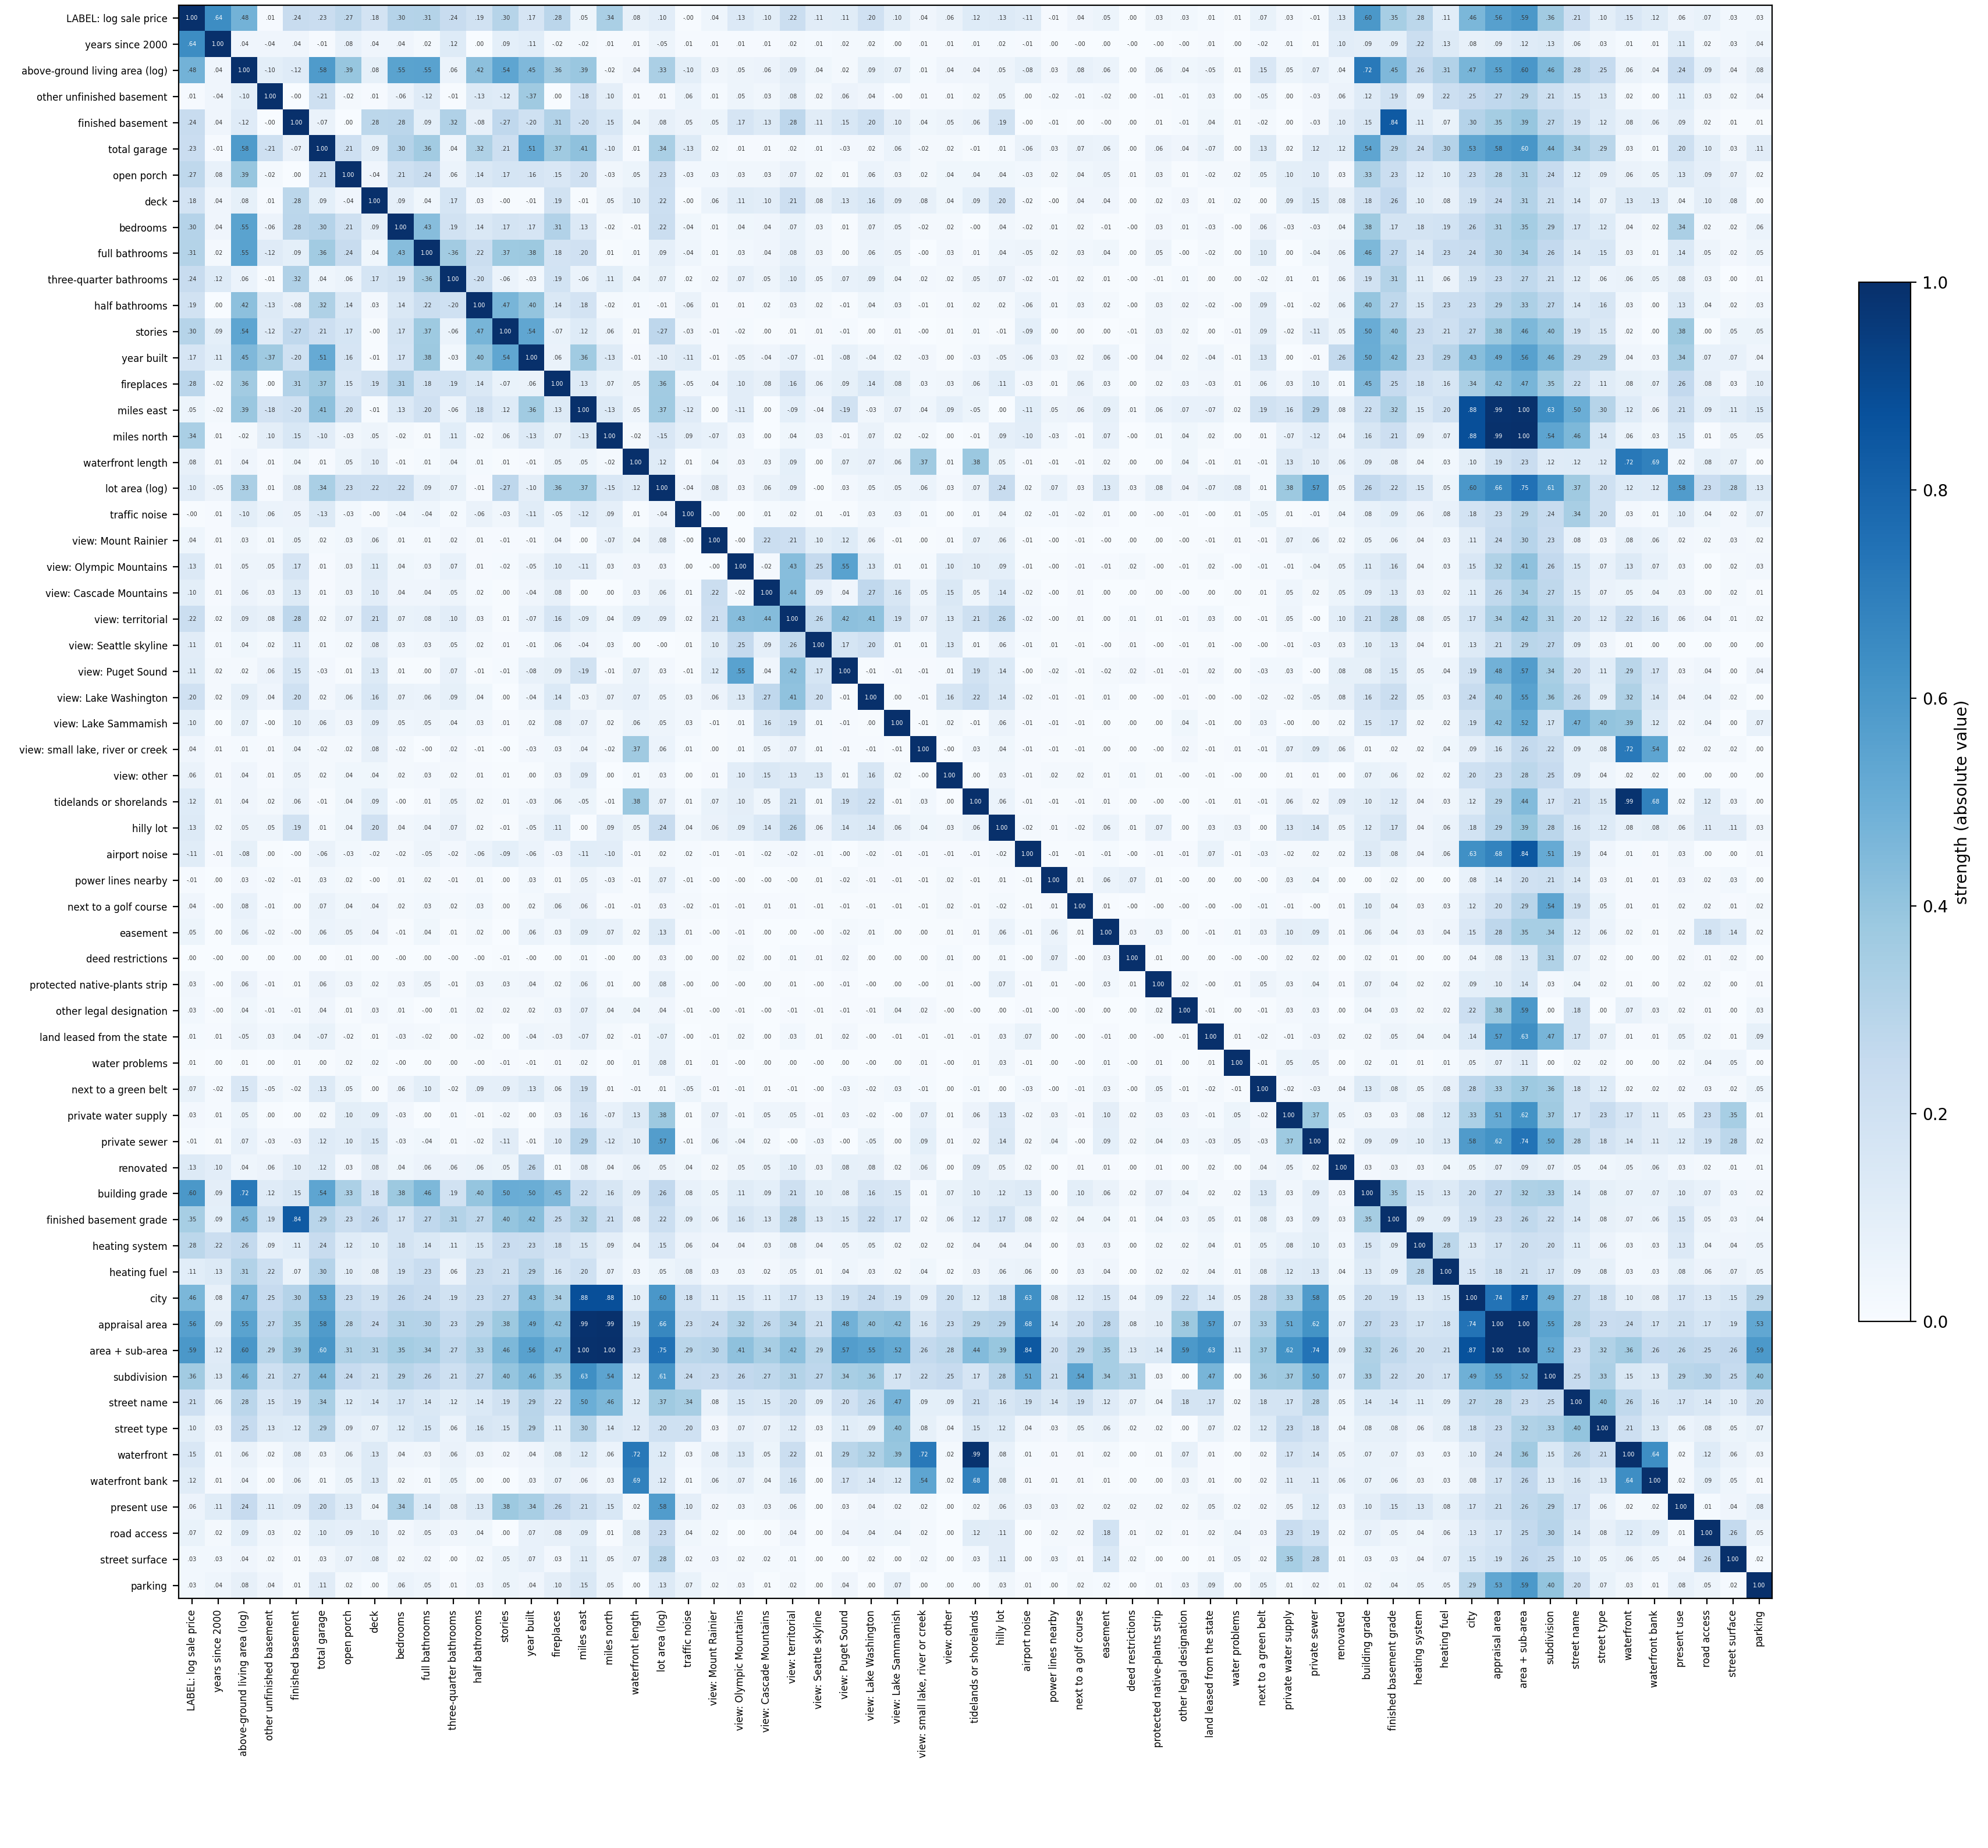
\includegraphics[width=\textwidth]{figures/correlation_heatmap.png}
\caption{Association between the label and the 60 candidate features on the training sales: Pearson correlation for two numbers, correlation ratio on held-out homes for a category and a number, bias-corrected Cram\'er's V for two categories.}
\label{fig:heatmap}
\end{figure*}

\end{document}
